% ****** Start of file aipsamp.tex ******
%
%   This file is part of the AIP files in the AIP distribution for REVTeX 4.
%   Version 4.1 of REVTeX, October 2009
%
%   Copyright (c) 2009 American Institute of Physics.
%
%   See the AIP README file for restrictions and more information.
%
% TeX'ing this file requires that you have AMS-LaTeX 2.0 installed
% as well as the rest of the prerequisites for REVTeX 4.1
%
% It also requires running BibTeX. The commands are as follows:
%
%  1)  latex  aipsamp
%  2)  bibtex aipsamp
%  3)  latex  aipsamp
%  4)  latex  aipsamp
%
% Use this file as a source of example code for your aip document.
% Use the file aiptemplate.tex as a template for your document.
\documentclass[aip,nobalancelastpage,
twocolumn,
%sd,%
rsi,%
 amsmath,amssymb,
%preprint,%
 reprint,%
%author-year,%
%author-numerical,%
]{revtex4}

\usepackage{float}
\usepackage{amsfonts}
\usepackage{algorithm}
\usepackage{algpseudocode}
\usepackage{graphicx}% Include figure files
\usepackage{dcolumn}% Align table columns on decimal point
\usepackage{listings}
\usepackage[utf8]{inputenc}
\usepackage{subfigure}
\usepackage[english]{babel}
\usepackage{bm}% bold math
\usepackage{verbatim}
\usepackage{hyperref}
\usepackage{xcolor}

%\usepackage[mathlines]{lineno}% Enable numbering of text and display math
%\linenumbers\relax % Commence numbering lines



\begin{document}

\preprint{AIP/123-QED}

\title{Project 5: Approximating the Ground State Energy in a Quantum Dot}

\author{Noah Oldfield}

\affiliation{ 
Department of physics, University of Oslo%\\This line break forced with \textbackslash\textbackslash
}%

\date{\today}% It is always \today, today,
             %  but any date may be explicitly specified

\begin{abstract}
The report studies the approximated ground state energies of a quantum dot consisting of two electrons under two trial wavefunctions $\Psi_{T1}$ and $\Psi_{T2}$. Part I studies the first trial function and performs stability computations in addition to approximating the ground state energy. The ground state energy was approximated by VMC, for a pure harmonic oscillator, to a $100\%$ degree of accuracy, while by adding a e-e repulsive perturbation; the ground state was approximated by VMC to deviate from the exact result by approximately 5.70\%. In part II this deviation is shown to be reducible by replacing the trial wavefunction with one which takes the cusp-condition into account, and by varying two variational parameters. The deviation
was found to be reducible to approximately 4.62\%. Lastly, in part III the virial theorem is studied under $\Psi_{T2}$ with optimal variational parameters; for both perturbed and unperturbed Hamiltonians. It was found that the e-e repulsion dominates for at and around the harmonic oscillator frequency $\omega= 0.42$ and that for larger frequencies, the system tends to behave more like a pure harmonic oscillator.
\end{abstract}
\maketitle


\section{Introduction}
Since it's publication in 1953, the paper titled \textit{Equation of State calculations using fast machines } has seen many new applications. A particular problem which the algorithm found its way into, was of quantum mechanical computations with many body systems, using the variational principle. A principle which will be introduced in the theory section. In short, the variational principle says that the expectation value of a quantum system's Hamiltonian, is greater than or equal to the system's ground state energy. If the wave function used for this computation, the so called \textit{trial wavefunction or simply trial function}, is large-dimensional and unknown; the computations may become increasingly difficult. They may even be impossible to perform without approximation methods. It is for computations such as this that the metropolis algorithm was designed to resolve. What it does, in essence, is make possible a sampling from \textit{any} probability distribution. Often so, very efficiently. \par

The supposed first application of the combined metropolis variational principle method (known formally as the variational Monte Carlo method, or VMC), came about in 1965. It was by William L. McMillan, with the paper titled \textit{Ground state of Liquid $He^4$}. In the paper, he manages to compute the ground state of liquid Helium-4 to within 20\% of the experimental value\cite{McMillanPaper} using VMC. Which is, from today's standards, not too accurate; but in light of the fact that this was in 1965, where computational methods had just been developed and lacking the necessary computational resources it was a very important application of the potential of VMC. One of McMillan's flaws were that the potential he used to described the Helium-Helium interactions, was taken to be the Lennard-Jones potential. Which is now a legacy approximation to the problem, and similar ones. \par

\begin{figure}[H]
\center
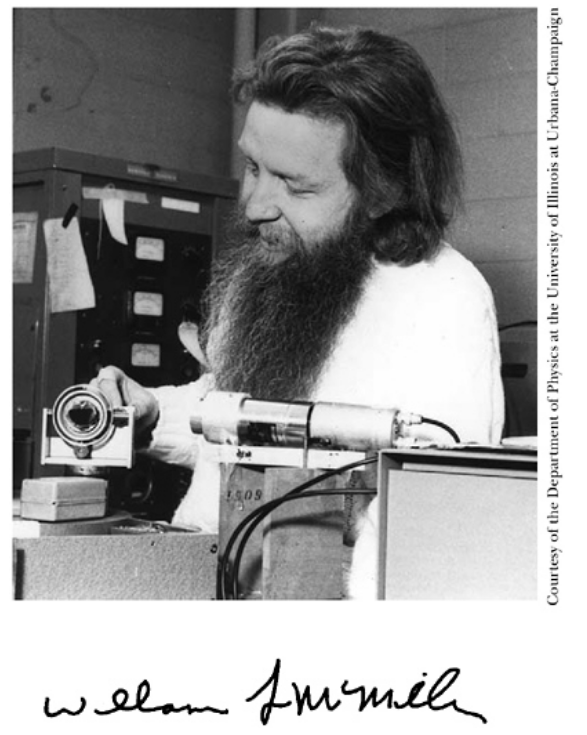
\includegraphics[scale=0.3]{mcmillan.png}
\caption{William L. McMillan. Picture reference \textit{$https://www.nap.edu/read/10470/chapter/12\#200$}}
\end{figure}

The reader of this report, is assumed to have knowledge equivalent to a completed university level course in quantum mechanics.\par
In this report, the VMC method will be applied to a system known as a quantum dot, this one consisting of two electrons. In reality a quantum dot is a nano-crystal, sized typically in the range $(2,10)nm$. The quantum dots have seen large scale modern applications, particularly within the color improvements of LED TV's. A nano-crystal such as a quantum dot, can thus be described quantum mechanically as a system of two electrons, confined in an isotropic (equal in every direction), three-dimensional harmonic oscillator potential. 
The electrons have both translational kinetic energy $T$, and potential energy $U$. The latter is a term which is actually comprised of two other terms, which in turn are due to two different physical effects. The first of these effects is the potential energy, which is due to the harmonic oscillator potential. The other is due to the Coulomb interaction between the electrons (electromagnetism). \par
This can also be viewed, in time-independent perturbation theory as having a system of two equal, three dimensional isotropic harmonic oscillators; where the electrons don't interact. This described as the unperturbed Hamiltonian with only the kinetic and potential oscillator term. While later effect consists of the electron-electron repulsion (or short e-e repulsion) interaction. Which, again, can be viewed as a perturbation to the pure harmonic oscillator system. However, perturbation theory is not a topic relevant for this project; it is only the technical terms: perturbed and unperturbed, which will be used to refer to the Hamiltonian with and without the e-e repulsion.\par

Since the VMC method applies the quantum mechanical variational method, a trial function is needed. Which is a wavefunction of the general form $\Psi(\vec{R};\alpha)$, where $\vec{R}$ are positional arguments, and $\alpha$ may also be a vector of so-called variational parameters. These variational parameters can be varied, as their name suggests, in order to tweak the wavefunction into a more suitable wavefunction for the system. Thus, the ground state energy of the system will be approximated using the VMC method with two different trial functions, named $\Psi_{T1}$ and $\Psi_{T2}$. The report itself is divided into three parts: I,II and III. In part I the threshold for thermalization, at which the system's properties, such as energy, can be sampled. Furthermore, the first trial function will be used to approximate the ground state energy of the quantum dot as both a perturbed and unperturbed system by VMC computations. The first trial function does not account for the cusp of the wavefunction itself, due to the e-e repulsion. It is a condition known as the cusp-condition. In order for the wavefunction to be properly normalized according to the first postulate of quantum mechanics, it must not diverge to infinity at any point. Else the probability distribution of the system is not well-defined. Part II will follow up on the computations of part I, but now using trial function 2, which introduces a new variational parameter. In whole $\Psi_{T2}$ accounts better for the cusp-condition than $\Psi_{T1}$ by introducing a so-called Jastrow factor. The best variational parameter found in part I will now be fixed in the computation and the new variational parameter will be computed to properly minimize the energy under the variational method. In the final part, part III, the virial theorem will be tested for the latter wavefunction under both perturbed and unperturbed conditions.\par

The author of this report has written another project, which applies the Metropolis algorithm to solve the Ising model, which might be useful to read if the reader is not very familiar with the application of the Metropolis algorithm\cite{Project4}. 


\section{Theory}
\subsection{Monte Carlo Integration}
The one dimensional integral

\begin{equation}
\label{simpleIntegration}
I = \int_a^b f(x) dx
\end{equation}

can be approximated using a stochastic approach

\begin{equation}
I \approx \frac{h}{N}\sum_{i=1}^N f(x_i)
\end{equation}

where: $h=b-a$ is the width of the integration interval, $N$ being the total number of integration points and $x_i$ is being sampled randomly from a uniform distribution $(a,b)$. For example, the integration of $f(x)=x^2$ from $a=0$ to $b=1$ would involve evaluating the function at a randomly assigned value in the interval $(0,1)$, and multiplying with the width $h$. This yields a very crude approximation by itself, but by repeating this process $N$ times with $N$ sufficiently large and by taking the mean. It would become better and better approximated to $I$.\par 
Since this is nothing but a \textit{sample} from an infinitely large distribution of other means, the error goes as the standard error. The standard deviation divided by the square root of $N$. Which means the error tends inversely with the square root of $N$

\begin{figure}[H]
\center
\caption{Example of the Monte Carlo Integration $\int_1^3 (x^2+3)dx$}
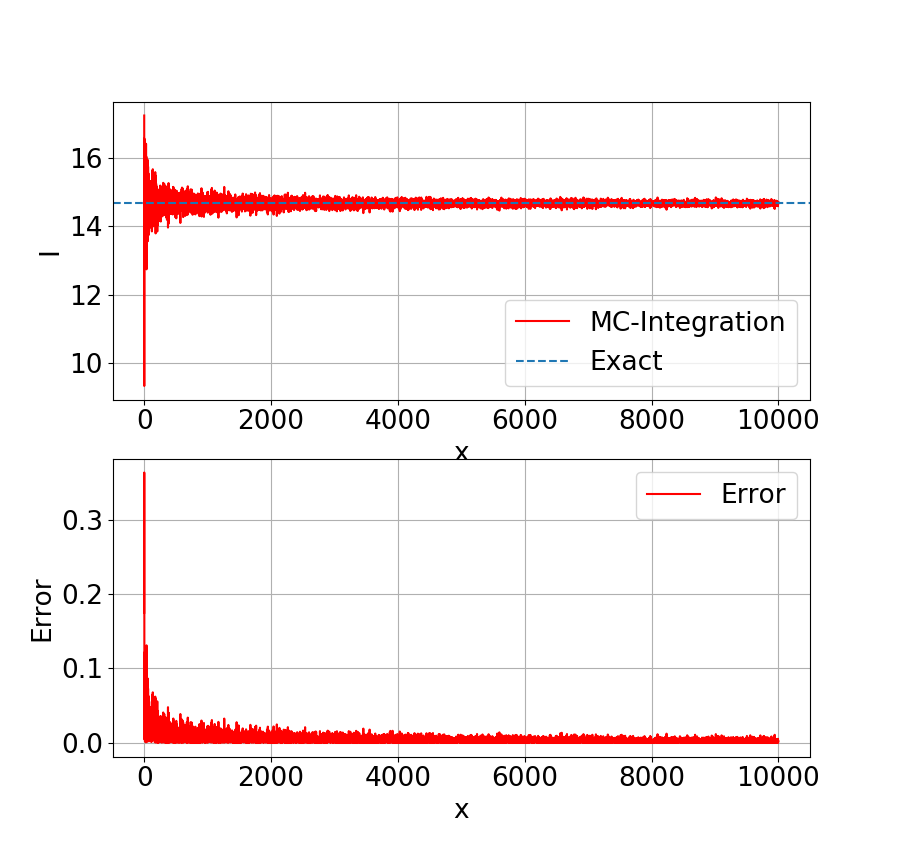
\includegraphics[scale=0.4]{mcint.png}
\end{figure}

\subsection{Importance Sampling}

When performing a Monte Carlo integration, there is a risk of acquiring numerous samples from a specific point which gives a significant increase in the variance, as opposed to other points in the integration domain. The method of importance sampling is thus a means to avoid this by sampling from a different, yet similar distribution to the original. The idea is to let the new distribution act as a weight function. The integration (\ref{simpleIntegration}) can be rewritten in terms of the weight function as 

\begin{equation}
I = \int_a^b \frac{f(x)}{g(x)} g(x) dx
\end{equation}

which, in statistical terms, conforms with computing the expected value of $f(x)/g(x) \equiv h(x)$, sampling from the probability distribution $g(x)$. \par
The variance $\sigma^2$ is thus
\begin{equation}
\sigma^2 = \int_a^b \left[h(x)\right]^2 g(x) dx - \left(\int_a^b h(x) g(x) dx\right)^2
\end{equation}

and if the weight function is chosen to be similar enough to f; the ratio of them will be approximately constant. Resulting in $h(x)=constant$ and going outside the integral

\begin{equation}
\lim_{ g(x) \to f(x)}  \sigma^2 = \left[h(x)\right]^2 -\left[h(x)\right]^2 = 0
\end{equation}

This shows the idea/method of importance sampling. The goal is to choose $g$ such as to be similar to $f$, but to cover certain areas which reduce the error introduced by the stochastic sampling of the Monte Carlo integration. For values in the integration domain which introduce large error, the weight function must be small, so as to minimize the error. 

\subsection{Metropolis Algorithm}
Referring to previously written project\cite{Project4}.\par 
The Metropolis algorithm is, in short, at its core, a method which enables sample-extraction from \textit{any} probability distribution. By technical terms of random walks. It is nicely visualized as walking through a probability distribution, \textit{favouring} steps which lead to higher probabilities.\par
The gist of the Metropolis algorithm will be implemented in the subsection together with the variational Monte Carlo method.


\subsection{The Variational Principle}
The variational principle yields an upper bound for the ground state energy $E_{gs}$, of a quantum system described by a Hamiltonian operator $\hat{H}$.

\begin{equation}
\label{VariationalPrinciple}
E_{gs} \leq \langle \psi| \hat{H} | \psi \rangle = \langle H \rangle
\end{equation}

for \textit{any} normalized wavefunction $\psi$, referred to, as in the introduction, as a \textit{trial wavefunction} or \textit{trial function}. 
\par More about the variational principle, and the proof can be found in Griffiths introductory textbook\cite[pg.293]{Griffiths}.\par

\subsubsection{The Variational Method}

The principle is very useful, since the majority of quantum mechanical systems are only solvable numerically. If the expectation value of the Hamiltonian can be computed analytically or numerically, then an interesting question is how close can one get to the exact ground state by minimizing $\langle H \rangle$? This is what is known as the variational method. Obviously, if the trial wavefunction \textbf{is} the exact ground state eigenstate for the system, then the inequality in (\ref{VariationalPrinciple}) becomes an equality.

\begin{equation}
\langle \psi| \hat{H} | \psi \rangle = \langle \psi| E_{gs} |\psi \rangle = E_{gs}\langle\psi | \psi \rangle = E_{gs}
\end{equation}

If not,however, there is no guarantee that the minima of $\langle H \rangle$ for the trial function equals the ground state energy; but the difference between the actual ground state energy and the approximated energy is minimized. How close the numerical solution will actually be to the actual ground state will then depend on the quality or the similarity of the trial function to the actual wavefunction.\par


\subsection{Quantum Many-body Systems }
As mentioned in the introduction, more broadly the wave function for a many body quantum mechanical system containing $N$ particles become a function of each individual particle's position $\vec{r}_i$ $i=1,2,3,\cdots, N$. Thus the wavefunction has a $3N$ dimensional spatial domain, if each particle is three dimensional. 
\begin{equation}
\Psi \rightarrow \Psi(\vec{r}_1,\vec{r}_2,\cdots, \vec{r}_N)=\Psi(\vec{R})
\end{equation}
The quantum dot system is thus described by a true wavefunction consisting of two such positional vectors, one for each electron, making it 6-dimensional.

\subsection{\label{sec:TheoryVirial }The Virial Theorem}
The virial theorem is originally a classical result which states that the relationship between the time averaged kinetic energy stable system and the potential energy is

\begin{equation}
\label{VirialTheorem}
\langle T \rangle = \frac{1}{2}\langle \vec{r} \cdot \nabla U\rangle
\end{equation}
a source with a good derivation of the theorem can be found in cited lecture notes from the university of Oklahoma\cite{VirialTheoremProof}.
The theorem, however, can be proved to hold in its classical form also for quantum mechanical systems, using Ehrenfest's theorem, which relates classical observables to their respective quantum expectation values.\par

For a system under a $n'th-degree$ exponential potential, the virial theorem states 
\begin{equation}
2\langle K \rangle = n\langle U\rangle
\end{equation}
thus for a simple harmonic oscillator, such as the unperturbed Hamiltonian $n=2$, the theorem becomes

\begin{equation}
\langle K \rangle = \langle U\rangle
\end{equation}
while for a system under a potential which goes as $1/r$, such as the perturbational term of to the Hamiltonian, the theorem states

\begin{equation}
2\langle T\rangle = \langle U \rangle
\end{equation}

\section{Numerical Method}
Presenting main numerical method for computations on the quantum dot system. The total number of Monte Carlo cycles for a given computation might be referred to as the \textit{cycle number}.

\subsection{\label{sec:theoryPhyssyst}Physical System Description and properties}
\begin{figure}[H]
\center
\caption{Geometric Illustration of the unperturbed Quantum Dot System under trial function $\Psi_{T1}$.}
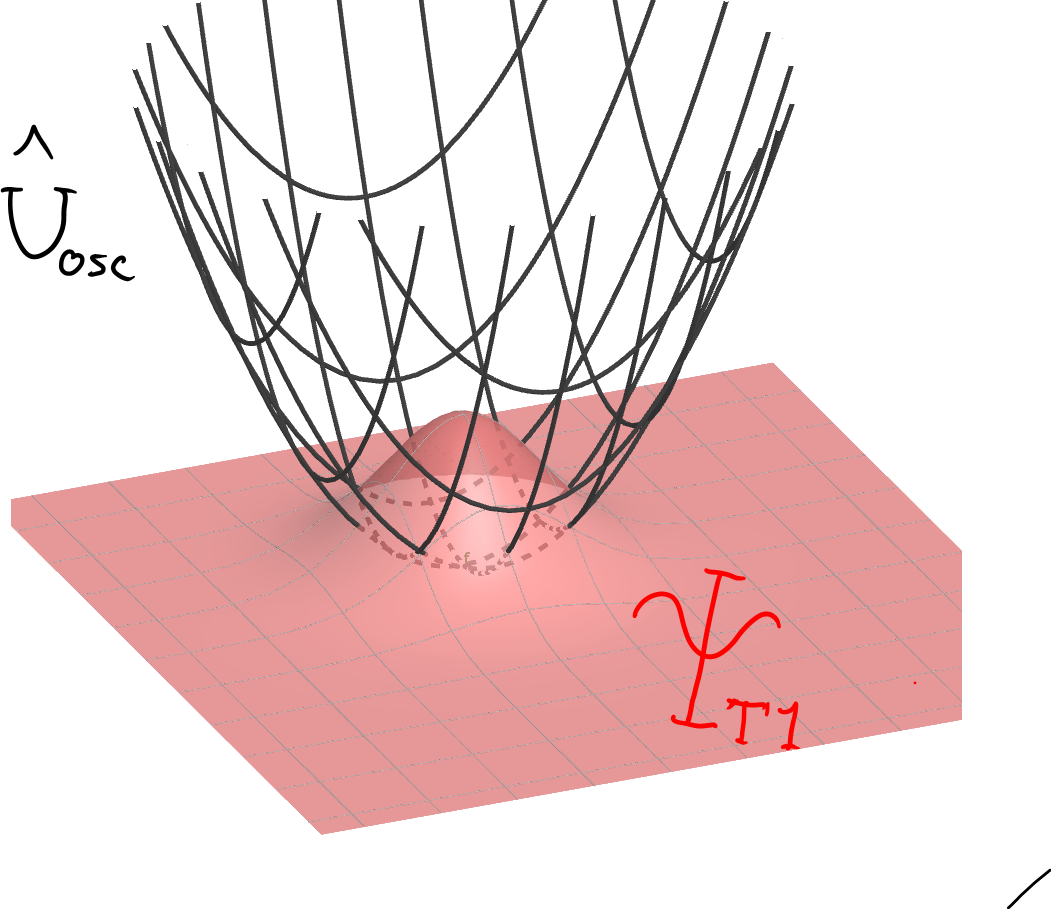
\includegraphics[scale=0.4]{probDist.png}
\end{figure}

The system is comprised of two electrons, confined in a pure three-dimensional isotropic harmonic oscillator
under the Hamiltonian

\begin{equation}
\label{Hamiltonian}
\hat{H} = \sum_{i=1}^2\left( -\frac{1}{2}\nabla_i^2 + \frac{1}{2}\omega^2 r_i^2\right) +\frac{1}{\left|\vec{r}_1 - \vec{r}_2\right|}
\end{equation}
the latter term is what shall be referred to as the perturbation $\hat{H}^1$, representing the e-e repulsion between the electrons. The first term with the sum is the unperturbed Hamiltonian $\hat{H}^0$. The latter term in the unperturbed Hamiltonian is the harmonic oscillator potential, while the first is the kinetic energy. The distance between the electrons will be abbreviated $r_{12}=\left|\vec{r}_1-\vec{r}_2\right|$.\par
When it comes to the total spin $s$ of the two electrons, each with spin $s_1=s_2=1/2$. They can combine, according to the Clebsch-Gordan table as total spin states with $s=0,1$, where there are three states corresponding to total spin 1 and only one state corresponding to total spin 0. The positional wave function for the unperturbed quantum dot system is known to be

\large
\begin{equation*}
\Phi(\vec{r}_1,\vec{r}_2)=Ce^{-\omega^2(r_1^2+r_2^2)/2}
\end{equation*}
\normalsize

and due to the Pauli-Exclusion principle, the total wave function which consists of the positional state and total spin state (or more generally total angular momentum) must be antisymmetric under exchange of particle labels. I.e the state must be an eigenstate of the parity operator with eigenvalue -1. \cite[pg.128]{Zettili}. \par
As seen the positional wave function is symmetric 
\begin{equation}
\hat{\mathcal{P}}\Phi(\vec{r}_r,\vec{r}_2) = 1\Phi(\vec{r}_2,\vec{r}_2)
\end{equation}
demanding that in order for the total wave function to be antisymmetric, it is the total spin state which needs to be antisymmetric, which means the only state which fulfills this is the state with total spin 0
\begin{equation}
|s=0\rangle = \frac{1}{\sqrt{2}}\Big(|\uparrow_1 \downarrow_2\rangle - |\downarrow_1 \uparrow_2 \rangle \Big)
\end{equation}
where the up/down states are labelled by particle 1 and 2. Combining this with the positional state, yields an antisymmetric wave function. Thus the electrons must be in a singlet spin state, with total spin $s=0$.


\subsection{Variational Monte Carlo}
The variational Monte Carlo method (VMC) is a conglomerate of the mentioned topics. It applies the variational method to approximate the ground state in a system. \par
Letting the variational principle (\ref{VariationalPrinciple}) being the initial base for the method, and dubbing the trial wave function $\Psi_T$, with implicit dependence upon the positions $\vec{R}=(\vec{r}_1,\vec{r}_2)$ and variational parameters $\alpha$.\par

In order to set up an efficient algorithm, importance sampling can be applied when computing the expectation value of the Hamiltonian, now allowing the trial wave function to not be normalized 

\begin{equation*}
\langle H \rangle = \frac{1}{\langle \Psi_T | \Psi_T \rangle}\int d\vec{R} \; \Psi_T^* \hat{H} \Psi_T 
\end{equation*}

\begin{equation*}
= \frac{1}{\langle \Psi_T | \Psi_T \rangle} \int d\vec{R} \; \Psi_T^* \left(\frac{\Psi_T^* \Psi_T}{\Psi_T^* \Psi_T}\right) \hat{H}\Psi_T
\end{equation*}

\begin{equation}
= \frac{1}{\langle \Psi_T | \Psi_T \rangle} \int d\vec{R} \; \left| \Psi_T\right|^2 \frac{1}{\Psi_T}\hat{H}\Psi_T 
\end{equation}

\begin{equation}
=  \int d\vec{R}\left(\frac{\left|\Psi_T\right|^2}{\langle \Psi_T | \Psi_T \rangle}\right)\; E_L = \int d\vec{R}\; \rho\;E_L
\end{equation}

where the term $E_L = \frac{1}{\Psi_T}\hat{H} \Psi_T$ is dubbed the local energy. From the importance sampling, this means that now positions can be sampled from the probability distribution of the system's trial wave function $\rho = \frac{\left|\Psi_T\right|^2}{\langle \Psi_T|\Psi_T\rangle}$ and used to evaluate the local energy. Effectively meaning that the expectation value of the Hamiltonian is equal to the expectation value of the local energy. Discretizing by Monte Carlo integration yields

\begin{equation}
\langle H\rangle =\langle E_L\rangle \approx \frac{1}{M} \sum_{i=1}^M E_L(\vec{R}_i) 
\end{equation}
where the sampling of $\rho$ is to be done by the Metropolis algorithm. \par



The full variational Monte Carlo algorithm is thus

\begin{algorithm}[H]
\caption{VMC Algorithm}
\label{VMCAlgorithm}
\begin{algorithmic}[1]
\State \textbf{FOR} $\mathcal{V} = \mathcal{V}_{min}, \mathcal{V}_{min}+h_\mathcal{V},\cdots, \mathcal{V}_{max} - h_\mathcal{V}, \mathcal{V}_{max}$
	\begin{itemize}
    \item Allocate $h_R$ such that the acceptance ratio $\sim 50\%$
    \item Initialize position $\vec{R}_{init}\in\{-5,5\}_{uniform}$
	\item Assign Storage-variables \par $\psi_{current}=\Psi_{T}(\vec{R}_{init};\mathcal{V})$  \&  $\vec{R}_{current} = \vec{R}_{init}$
   \State \textbf{FOR} $cycle = 1,2,\cdots , N_{MC}$
   \begin{itemize}
   \item Propose Translation \par
    $\vec{R}' = \vec{R}_{current} + h_R \cdot \left( \gamma \in \{-\frac{1}{2}, \frac{1}{2}\}_{uniform}\right)$
   \item Evaluate the Probability ratio \par
    $\mathcal{P}=\frac{\left|\Psi_T\left(\vec{R}';\mathcal{V}\right)\right|^2}{\left|\psi_{current}\right|^2}$\par
	\textbf{Metropolis Test}
   \item[] \textbf{IF}: $\mathcal{P}\geq \left(u \in \{0,1\}_{uniform}\right)$ \textbf{DO}: Accept Translation and Compute Expectation Values
   \item[] \textbf{ELSE}: \textbf{DO}: Reject Translation and Compute Expectation Values
   \end{itemize}
\end{itemize}
\State Choose $\langle E_L\left(\mathcal{V}_i\right)\rangle =$\par 
\small
$min\{\langle E_L\left(\mathcal{V}\right)\rangle, \langle E_L\left(\mathcal{V} + h_\mathcal{V}\right)\rangle,\cdots, \langle E_L\left(\mathcal{V}_{max}\right)\rangle$
\normalsize \par

\State Then $E_{gs} \approx \langle E_L\left(\mathcal{V}_i\right)\rangle$
   \end{algorithmic}
\end{algorithm}

here $\mathcal{V}$ denotes an arbitrary chosen variational parameter, all other variational parameters are held fixed at some chosen value for this report's purposes. Notice that $\mathcal{P}$ is not the parity operator mentioned in (\ref{sec:theoryPhyssyst}). Some subtleties must be mentioned. The step-size $h_R$ is, as seen in the algorithm, a step-size for translating the particles from one point in the distribution to another. One way of locating an optimal step-size (yielding $\sim 50\%$ acceptance ratio) is by running a separate \textit{low-quality} Metropolis-algorithm run for each variational iteration. What \textit{low-quality} implies, is a low total number of Monte Carlo cycles, and without all unnecessary calculations, such as expectation values of energy. Simply performing about $10^3$ cycles should give a very good estimate for the acceptance ratio and thus being quite efficient. A simple synopsis of an algorithm which performs this is thus
\begin{itemize}
\item Set initial $h_R=15$
\item while: condition (AcceptRatio NOT$\in$ some interval)
\item Run Metropolis-Algorithm with cycle number $10^3$
\item Reduce $h_R$ by specified value
\item Stops when condition is false
\end{itemize}

\subsection{\label{sec:Method:subsec:Part I}Part I: Trial Wave function}
Moving on to the computations for this report.\par

The first trial wave function for the computation is given as 


\begin{equation}
\label{TrialFunction1}
\Psi_{T1} = Ce^{-\alpha \omega(r_1^2 + r_2^2)/2}
\end{equation}

with which an analytical expression for the unperturbed local energy can be found. This is needed for the algorithm

\begin{equation}
\label{LocalEnergyUnperturbedSetup}
E_L = \frac{1}{\Psi_{T1}}\left( -\frac{1}{2}\nabla_1^2 -\frac{1}{2}\nabla_2^2 + \frac{1}{2}\omega^2 (r_1^2+r_2^2)\right) \Psi_{T1}
\end{equation}

\begin{equation}
\label{LocalEnergyUnperturbedSetup2}
=\frac{1}{\Psi_{T1}}\left( -\frac{1}{2}\nabla_1^2 -\frac{1}{2}\nabla_2^2\right)\Psi_{T1} + \frac{1}{2}\omega^2 (r_1^2+r_2^2) 
\end{equation}

since the wave function is separable $\Psi_{T1} = \psi_1 \psi_2$, the laplacian acting on the wave function for a single particle $\psi = Ce^{-\beta r^2}$ (omitting particle labels) can be computed first. 

\small
\begin{equation*}
 \nabla^2 Ce^{-\beta r^2} = C\frac{1}{r^2}\frac{\partial}{\partial r}\left(r^2 \frac{\partial}{\partial r} \right) e^{-\beta r^2}= -2\beta C \frac{1}{r^2}\frac{\partial}{\partial r}\left(r^3 e^{-\beta r^2}\right)
\end{equation*}

\begin{equation*}
= -2\beta C\frac{1}{r^2}\left(3r^2 e^{-\beta r^2} -2\beta r^4 e^{-\beta r^2}\right) = 2\beta C e^{-\beta r^2}\left(2\beta r^2 - 3\right)
\end{equation*}

\normalsize


finally
\begin{equation}
\label{term}
\nabla^2 \psi= 2\beta \left( 2\beta r^2 - 3\right)\psi
\end{equation}

which means that each laplacian acting on $\Psi_{T1}$ in (\ref{LocalEnergyUnperturbedSetup}) will result in (\ref{term}) multiplied by the separated wave function which is held constant during differentiation, for example $\nabla_1^2 \Psi_{T1} = \psi_2 2\beta (2\beta r_1^2 -3)\psi_1=2\beta (2\beta r_1^2-3)\Psi_{T1}$ with $\beta = \frac{\alpha \omega}{2}$.
Computing thus the first term in (\ref{LocalEnergyUnperturbedSetup2})

\begin{equation}
-\frac{1}{2}\left(\frac{1}{\Psi_{T1}}\nabla_1^2\Psi_{T1} + \frac{1}{\Psi_{T1}}\nabla_2^2\Psi_{T1}\right)
\end{equation}

\begin{equation}
= -\frac{1}{2}\left(2\beta\left(2\beta r_1^2-3\right) + 2\beta\left(2\beta r_2^2-3\right)\right)
\end{equation}

\begin{equation}
= -2\beta^2r_1^2 - 2\beta r_2^2 + 6\beta
\end{equation}
substituting $\beta = \frac{1}{2}\alpha \omega$ , it works out to

\begin{equation}
= -\frac{1}{2}\omega^2\alpha^2\left(r_1^2 - r_2^2\right) + 3\alpha \omega
\end{equation}
combining with the harmonic oscillator part in (\ref{LocalEnergyUnperturbedSetup2})

\begin{equation}
E_L = \frac{1}{2}\omega^2 (r_1^2 + r_2^2 - \alpha^2 r_1^2 - \alpha^2 r_2^2) + 3\alpha \omega
\end{equation}

\begin{equation}
\label{LocalEnergyT1UAnalytical}
E_L = \frac{1}{2}\omega^2 \left(r_1^2 + r_2^2\right) \left(1-\alpha^2\right) + 3\alpha \omega
\end{equation}

which gives the analytical expression for computing the local energy for the first trial function when the system is considered unperturbed (the e-e repulsion is disregarded). If, however, the e-e repulsion is to be taken into account, the extra term $1/r_{12}$ needs to be added to (\ref{LocalEnergyT1UAnalytical}), giving the analytical local energy for the perturbed case. Thus there is a requirement to differentiate between the local energies, in regards to if the system is being regarded perturbed or unperturbed. The sub-indices for these are respectively $T1P$ and $T1U$. Summarizing

\begin{align}
E_{LT1U} &= \frac{1}{2}\omega^2 \left(r_1^2 + r_2^2\right) \left(1-\alpha^2\right) + 3\alpha \omega \\
E_{LT1P} &= E_{LT1U} + \frac{1}{r_{12}}
\end{align}


This part will thus perform VMC calculations to find the best approximation for the unperturbed and perturbed system's ground state energies, using the trial wave function $T1$. The stability of the solutions can be studied by performing a series of VMC-s with varying number of Monte Carlo cycles  This is analogous to letting the system thermalize. After this is quantified, the expectation values can be computed after the system has thermalized. Thus using the variance of the local energy as a stability measurement. Hopefully this will yield an optimal variational parameter $\alpha$. \par
 Lastly, the expectation value of the distances between the particles $r_{12}$ will be studied for frequencies $\omega \in \{0.01, 0.5, 1.0\}$.


\subsection{Part II: Improved Trial Wave function}
In this part, only the perturbed system will be studied.\par
The second trial wave function of consideration is taken to account for the e-e repulsion by have an additional factor, known as a Jastrow factor. \par
The Jastrow factor is introduced as a means to handle the infinities which might arise during computation of expectation values. This is due to the perturbation term in the Hamiltonian (\ref{Hamiltonian}) when $r_{12}\to 0$. The Jastrow factor is thus a minimal requirement of the trial wave function in order to create the cusp for the wave function so that it can be properly normalized and thus be an element of the Hilbert space $\mathcal{H}$. I.e satisfying the first postulate of quantum mechanics\cite{LectureNotes}.

\large
\begin{equation}
\label{Trialfunction2}
\Psi_{T2}(\vec{R};\alpha,\beta) = C e^{-\frac{\alpha \omega}{2}\left(r_1^2 + r_2^2\right)}e^{\frac{r_{12}}{2\left(1+\beta r_{12}\right)}}
\end{equation}
\normalsize
This trial function is a function of the initial variational parameter $\alpha$ in addition to the new parameter $\beta$.\par
The computing of the analytical expression for the local energy is now a more comprehensive exercise. Although it is seemingly good exercise. One procedure for doing this is by using the law of cosines for expressing $r_{12}$

\begin{figure}[H]
\center
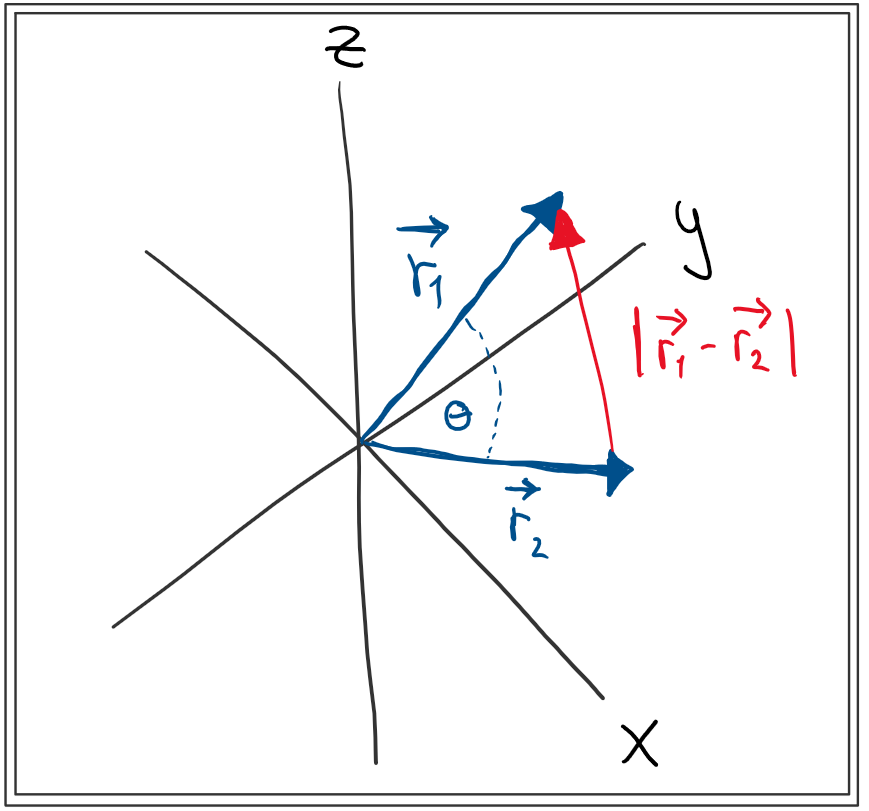
\includegraphics[scale=0.45]{axis.png}
\caption{Geometric illustration of the Cartesian position-space for applying the law of cosines. }
\end{figure}

as
\begin{equation}
r_{12} = \left|\vec{r}_1-\vec{r}_2\right| = |\vec{r}_1|^2 + |\vec{r}_2|^2 - 2\vec{r}_1 \cdot \vec{r}_2 \theta'
\end{equation}
\begin{equation}
= r_1^2 + r_2^2 -2r_1r_2 \theta'
\end{equation}

and using the product rule for differentiation of $\nabla^2 \left(\Psi_{T1} \psi'\right)$ where $\psi'$ equals the second factor in (\ref{Trialfunction2})

where $\theta'=\cos\theta$ is assumed constant.\par

The result is given as

\begin{equation*}
E_{LT2P} = E_{LT1P} 
\end{equation*}
\small
\begin{equation}
+ \frac{1}{2\left[g(r_{12})\right]^2}\left[\alpha \omega r_{12} -\frac{1}{2\left[g(r_{12})\right]^2} - \frac{2}{r_{12}}+\frac{2\beta}{g(r_{12})}\right]
\end{equation}
\normalsize
where $g(r_{12}) = 1+\beta r_{12}$

Now satisfying the cusp condition when $r_{12}\to 0$, it is expected to be a better physical representation for the system. The optimal variational parameter found for the first trial function is, as named, the optimal for this particular trial function, thus the new parameter $\beta$ will be varied in the coming computations. By doing this, one hope to acquire an even better approximation for the ground state energy. This process, can be repeated, going back to varying $\alpha$ and so forth.\par
When this process has been done such that varying the parameters yield no significant improvements, the optimal parameters will be considered to be found. \par
The same computation for the expectation value of the distance $r_{12}$ will be performed for varying frequencies, in the same interval, as in (\ref{sec:Method:subsec:Part I}).

\subsection{Part III: Virial Theorem}
In this part, the virial theorem will be tested by computing the kinetic and potential energy of the second trial function.  This will be done under the optimal parameters found in part II, and with cycle number equal to the most efficient in terms of accuracy and resources. The optimal variational parameters for $\alpha$ and $\beta$ will be applied in these calculations for both perturbed and unperturbed Hamiltonians.  \par
Also, as in parts I and II, the mean distance $r_{12}$ will be studied frequencies $\omega\in\{0.01,1.0\}$ for an appropriate frequency step-size. 

\section{Results}
\subsection{Part I: }
\textit{Results from this section found in folder bla bla}.\par
Firstly the stability is computed for the system under the unperturbed Hamiltonian.

\begin{figure}[H]
\center
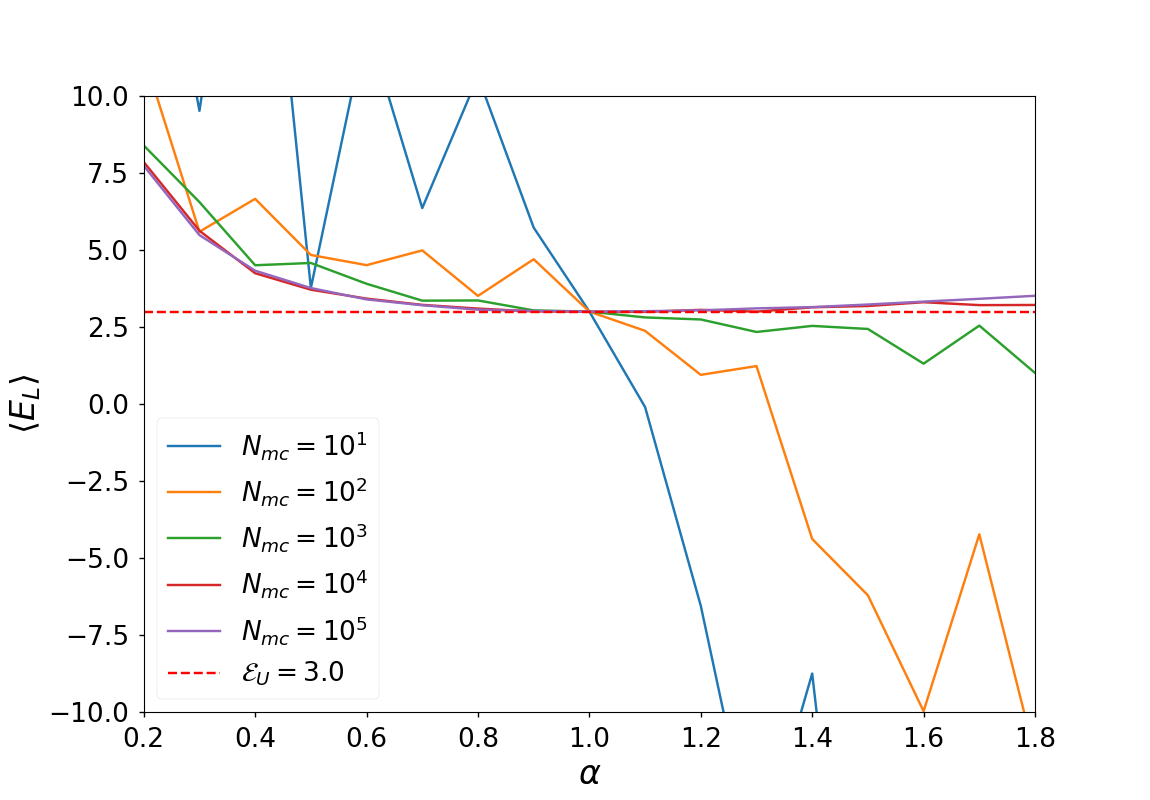
\includegraphics[scale=0.33]{figsPartI/IStabilityE.png}
\caption{Harmonic Oscillator Potential (Unperturbed).\newline Five VMC computations for increasing total number of Monte Carlo cycles $N_{mc}$. Expectation value of the local energy $\langle E_L \rangle$ as function of the variational parameter $\alpha$. Variational step-size $h_\alpha = 0.1$.}
\label{Ifig1}
\end{figure}
quantifying further with a plot of the variance $\sigma^2$ for each respective computation

\begin{figure}[H]
\center
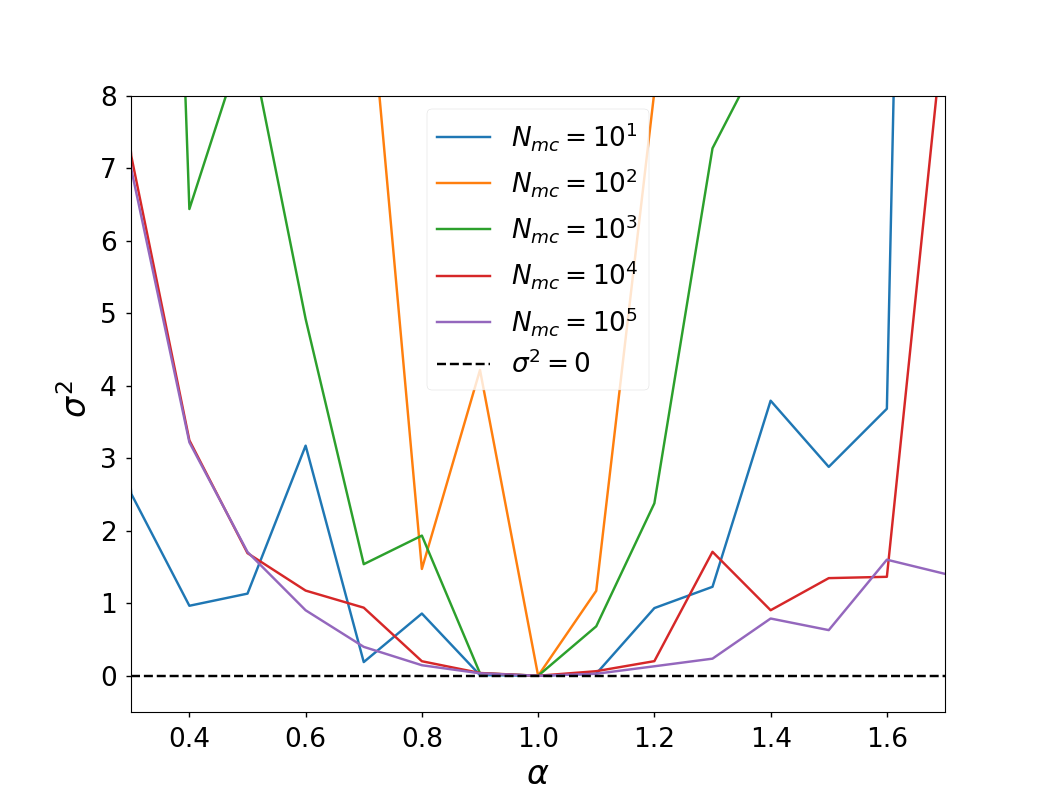
\includegraphics[scale=0.33]{figsPartI/IStabilitySigma.png}
\caption{Harmonic Oscillator Potential (Unperturbed).\newline Five VMC computations for increasing total number of Monte Carlo cycles $N_{mc}$. Variance $\sigma^2$ of the local energy $\langle E_L \rangle$ as function of the variational parameter $\alpha$. Variational step-size $h_\alpha = 0.1$.}
\label{Ifig2}
\end{figure}

this gives the thermilzation threshold for the system for which it has a defined minima, at about $N_{mc}=10^4$ total Monte Carlo cycles.
In addition to the thermilzed threshold, computing three further additionally after the thermalization threshold. \par

\begin{figure}[H]
\center
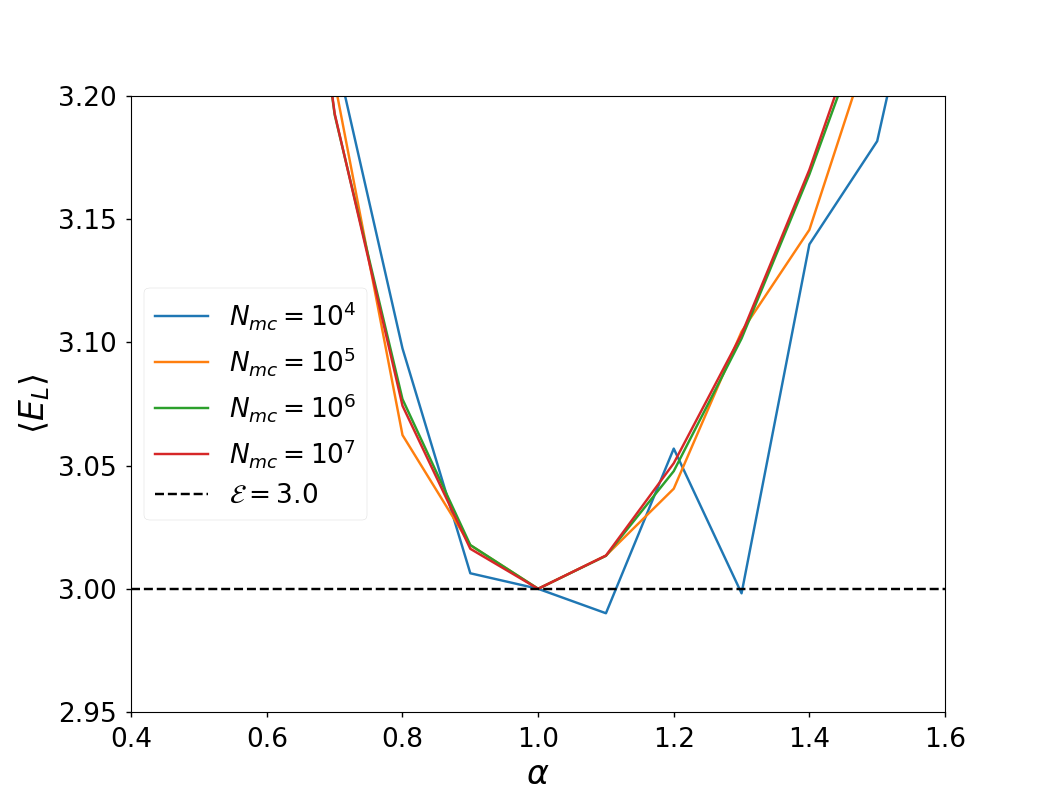
\includegraphics[scale=0.33]{figsPartI/IStabilityThermalizedE.png}
\caption{Harmonic Oscillator Potential (Unperturbed).\newline Three VMC computations for increasing total number of Monte Carlo cycles $N_{mc}=10^i$, i=4,5,6,7. Expectation value of the local energy $\langle E_L \rangle$ as function of the variational parameter $\alpha$. Variational step-size $h_\alpha = 0.1$.}
\label{Ifig3}
\end{figure}

as again, the variance is included 

\begin{figure}[H]
\center
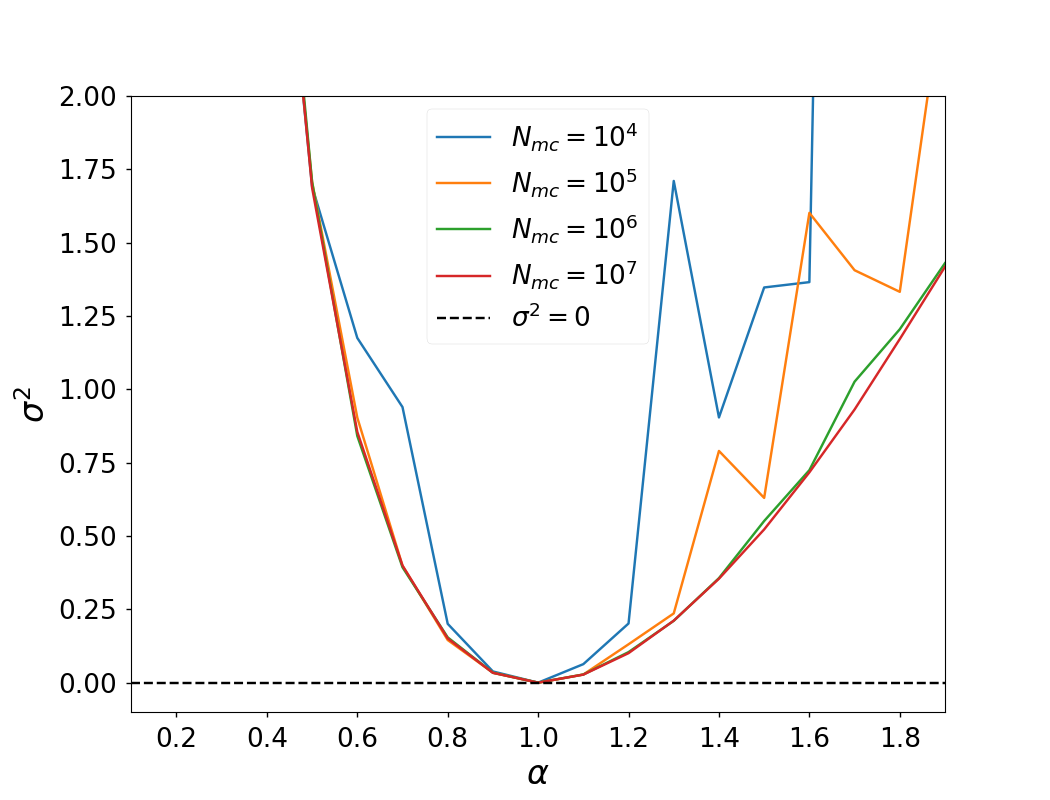
\includegraphics[scale=0.33]{figsPartI/IStabilityThermalizedSigma.png}
\caption{Harmonic Oscillator Potential (Unperturbed).\newline Three VMC computations for increasing total number of Monte Carlo cycles $N_{mc}=10^i$, i=4,5,6,7. Variance $\sigma^2$ of the local energy $\langle E_L \rangle$ as function of the variational parameter $\alpha$. Variational step-size $h_\alpha = 0.1$.}
\label{Ifig4}
\end{figure}

the minimum local energy for all thermalized computations are thus 

\begin{table}[H]
\center
\caption{Minimal value of the local energy $\langle E_L\rangle_{min}$ for the associated total number of Monte Carlo cycles $N_{mc}$ and variational parameter.}
\begin{tabular}{| p{2cm} | p{2cm} | p{2cm} |}
\hline
$\alpha$ & $N_{mc}$ & $\langle E_L \rangle_{min}$ \\
\hline
$1.1$ & $10^4$ & $2.9901$\\
\hline
$1.0$ & $10^5$ & $3.0000$\\
\hline
$1.0$ & $10^6$ & $3.0000 $\\
\hline
$1.0$ & $10^7$ & $3.0000 $\\
\hline
\end{tabular}
\label{resItable1}
\end{table}

Now computing for the perturbed system, adding the electron electron repulsion

\begin{figure}[H]
\center
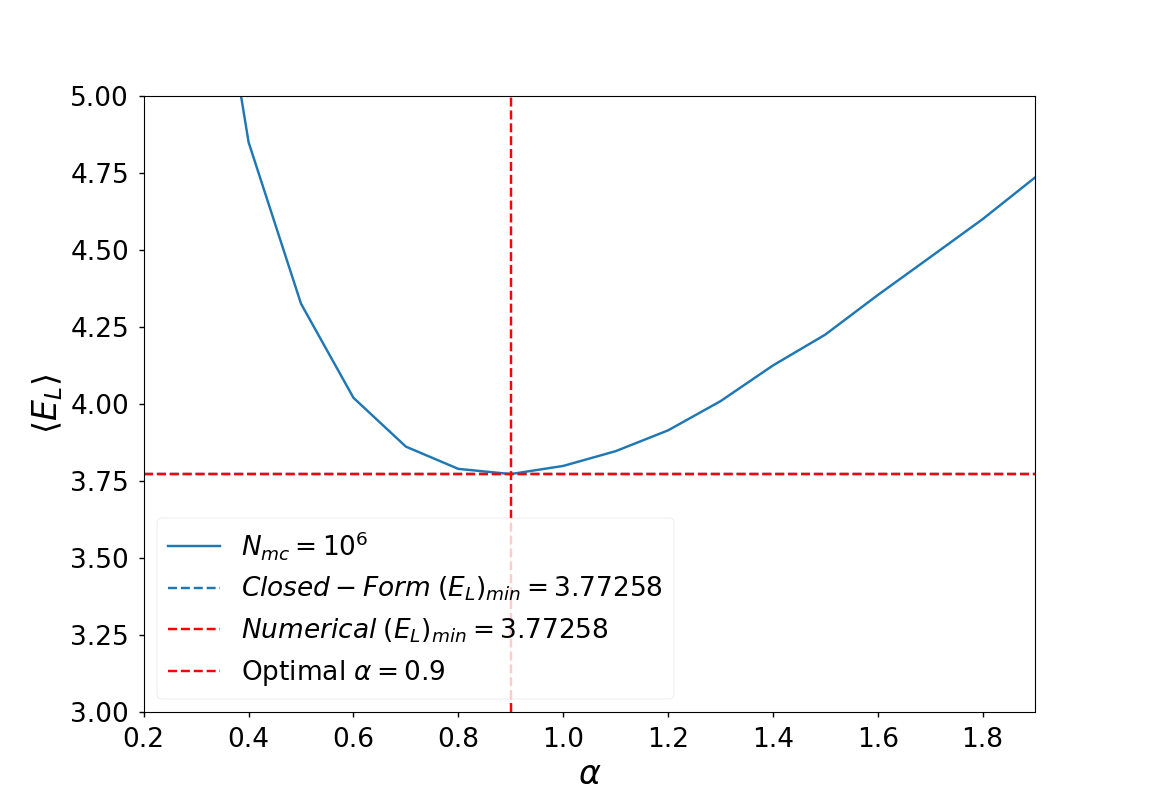
\includegraphics[scale=0.32]{figsPartI/IStabilityPertE.png}
\caption{Harmonic Oscillator Potential (Perturbed).\newline Single VMC computation of Monte Carlo cycles $N_{mc}=10^6$. Local energy $\langle E_L \rangle$ as function of the variational parameter $\alpha$. Variational step-size $h_\alpha = 0.1$.}
\label{Ifig5}
\end{figure}

also the variance

\begin{figure}[H]
\center
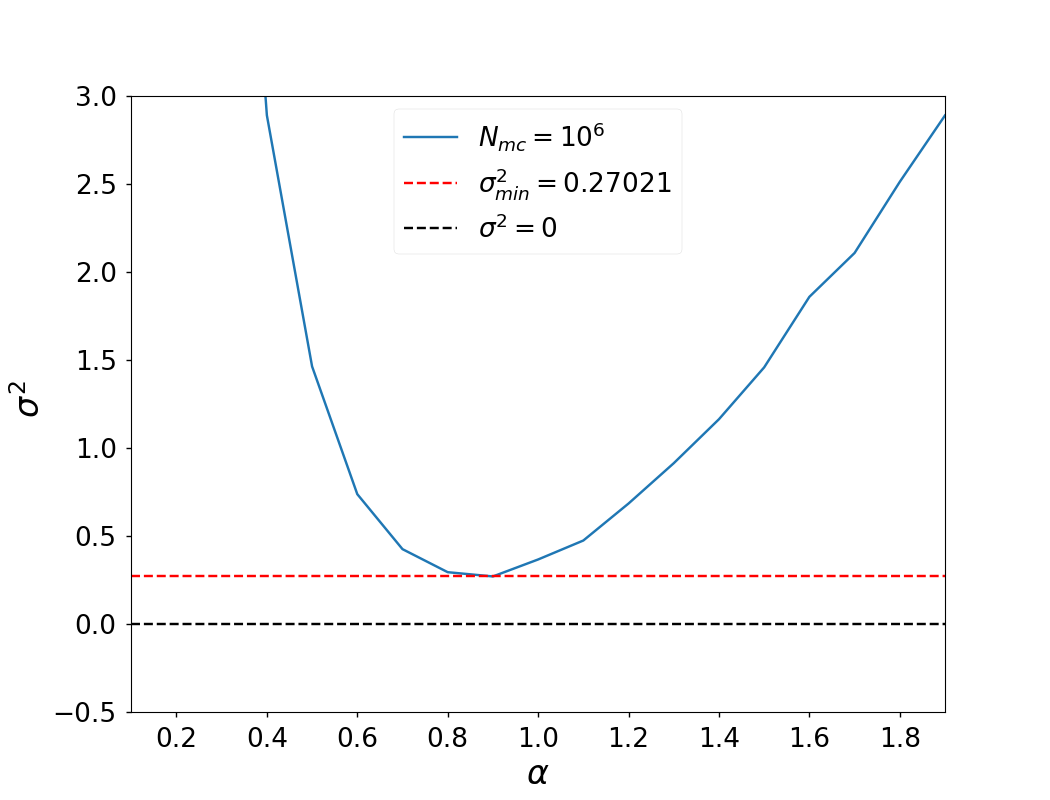
\includegraphics[scale=0.32]{figsPartI/IStabilityPertSigma.png}
\caption{Harmonic Oscillator Potential (Perturbed).\newline Single VMC computation of Monte Carlo cycles $N_{mc}=10^6$. Variance $\sigma^2$ of the local energy $\langle E_L \rangle$ as function of the variational parameter $\alpha$. Variational step-size $h_\alpha = 0.1$.}
\label{Ifig6}
\end{figure}

The results of the local energy computations for both perturbed and unperturbed Hamiltonians can be summarized

\begin{table}[H]
\center
\caption{Local energy minima $\langle E_L \rangle_{min}$, optimal variational parameter $\alpha$ and variance $\sigma^2$ for the perturbed and unperturbed Hamiltonians. Under trial function $\Psi_{T1}$.}
\begin{tabular}{| p{2cm} | p{2cm} | p{2cm} | p{2cm} |}
\hline
 & $\langle E_L \rangle_{min}$ & $\alpha$ & $\sigma^2$\\
\hline
Unperturbed & $3.000$ & $1.0$ & $0$\\
\hline
Perturbed   & $3.773\pm 10^{-3}$ & $0.9$ & $0.270$  \\
\hline
\end{tabular}

\end{table}

The standard error is computed by (ref).\par
The mean distance for both perturbed and unperturbed is shown for the optimal parameters $\alpha \in \{0.9,1.0\}$ for frequencies $\omega \in \{0.01, 0.5, 1.0\}$.

\begin{figure}[H]
\center
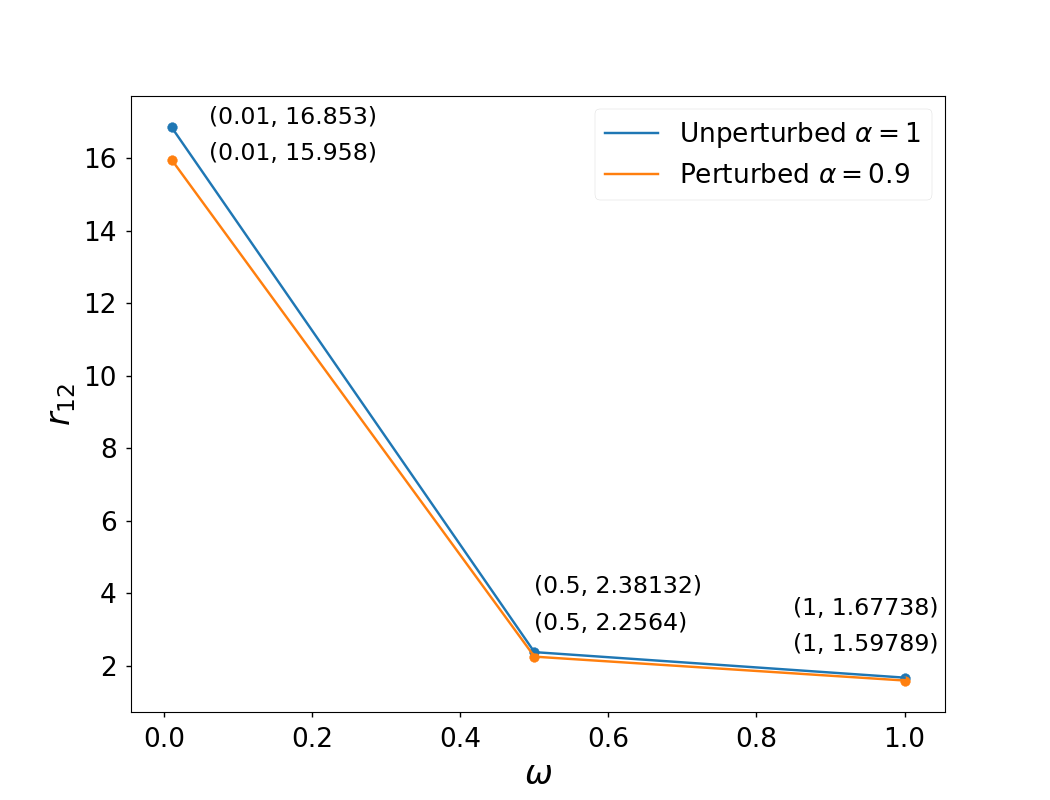
\includegraphics[scale=0.35]{figsPartI/IOmegas.png}
\caption{Harmonic Oscillator Potential (Perturbed).\newline Single VMC computation of Monte Carlo cycles $N_{mc}=10^6$. Variance $\sigma^2$ of the local energy $\langle E_L \rangle$ as function of the variational parameter $\alpha$. Variational step-size $h_\alpha = 0.1$.}
\label{Ifig7}
\end{figure}
the unperturbed distances are globally larger for the unperturbed computation

\begin{table}[H]
\center
\caption{Mean distances $r_{12}^{(i)}$ for perturbed ($i=U$) and unperturbed ($i=P$) Hamiltonians under varying frequencies $\omega$.}
\begin{tabular}{| p{2cm} | p{2cm} | p{2cm} |}
\hline
$\omega$ & $r_{12}^{(U)}$ & $r_{12}^{(P)}$\\
\hline
$0.001$ & $15.96$ & $16.85$\\
\hline
$0.5$   & $\phantom{1}2.26$  & $\phantom{1}2.38$\\
\hline
$1.0$   & $\phantom{1}1.60$  & $\phantom{1}1.70$\\
\hline
\end{tabular}
\label{TablePartI}
\end{table}


\subsection{Part II: }
Basing the computations on the optimal value of the perturbed system $\alpha=0.9$ found in result section I and computing 

\begin{figure}[H]
\center
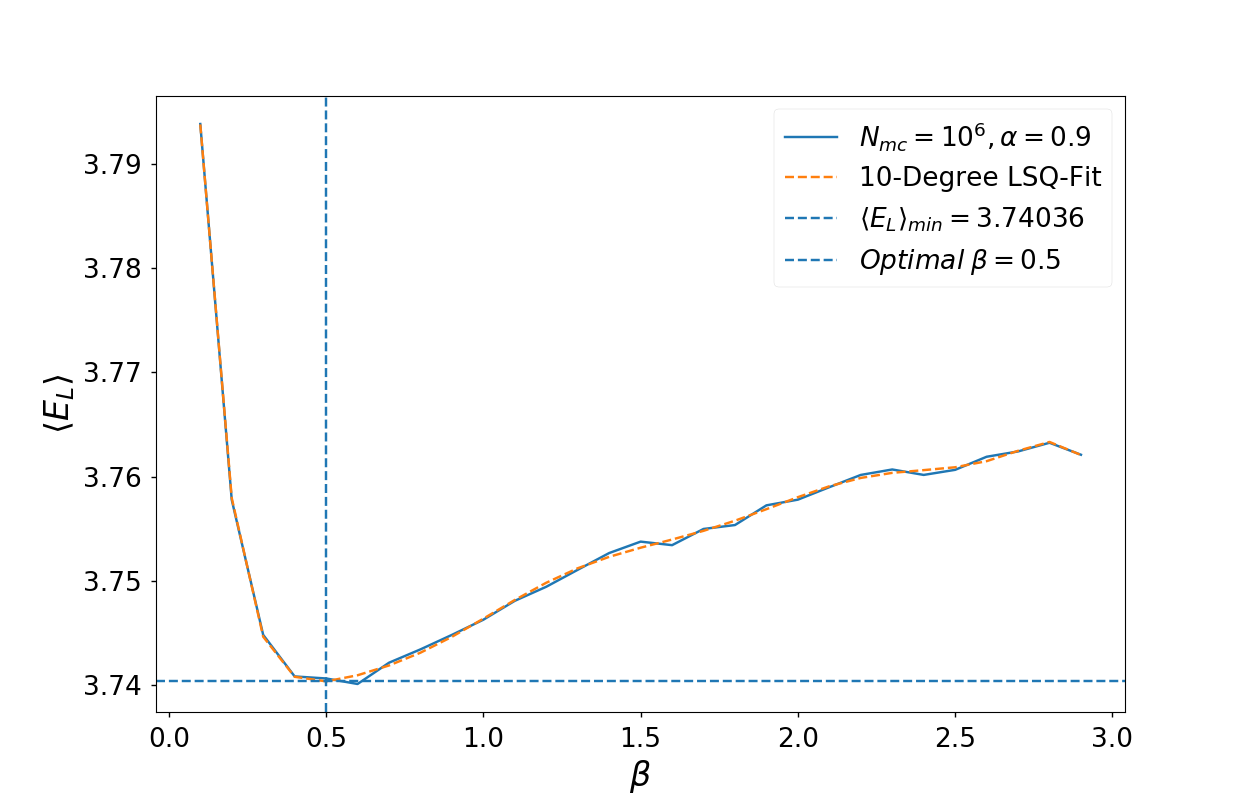
\includegraphics[scale=0.30]{figsPartII/run1.png}
\caption{Caption.}
\label{IIfig1}
\end{figure}

now minimizing under the the optimal $\beta = 0.5$

\begin{figure}[H]
\center
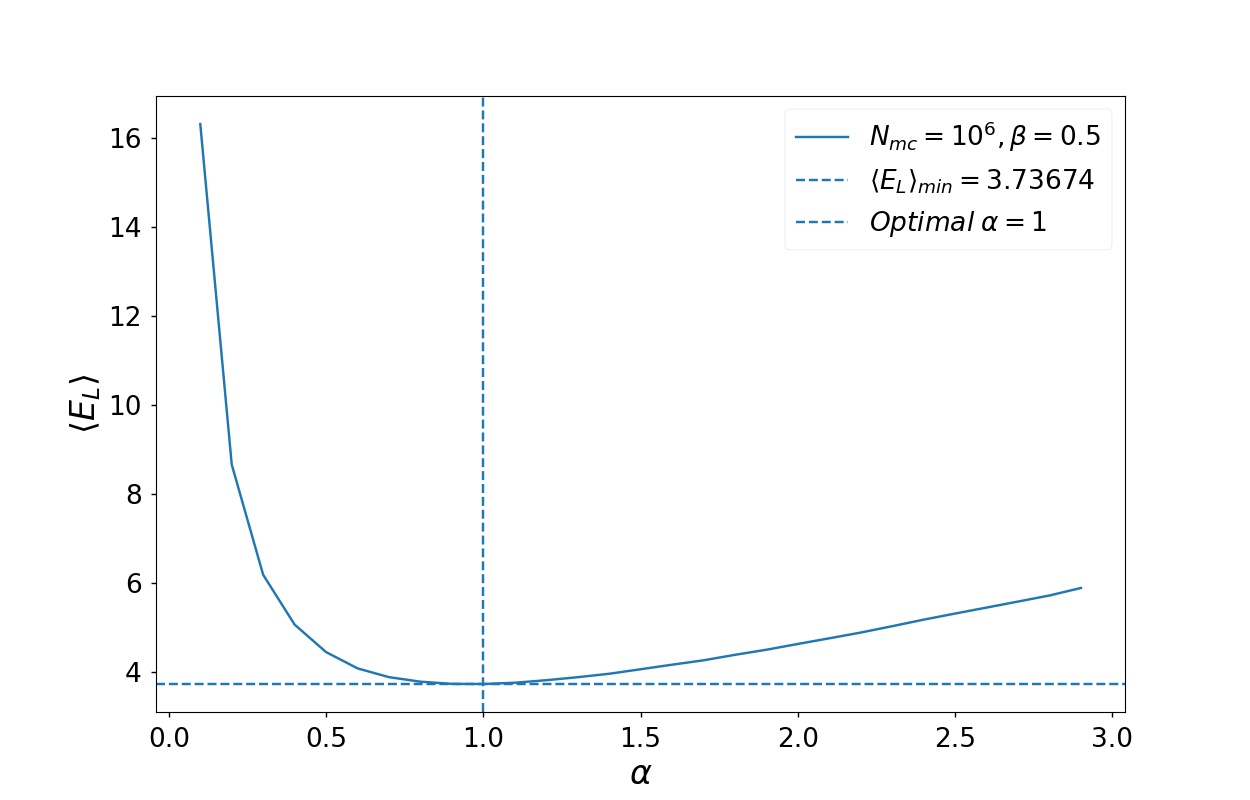
\includegraphics[scale=0.30]{figsPartII/run2.png}
\caption{Caption.}
\label{IIfig2}
\end{figure}

repeating the process (intermediatary runs found in folder \textit{$/project/figsPartII$}) eventually yields

\begin{figure}[H]
\center
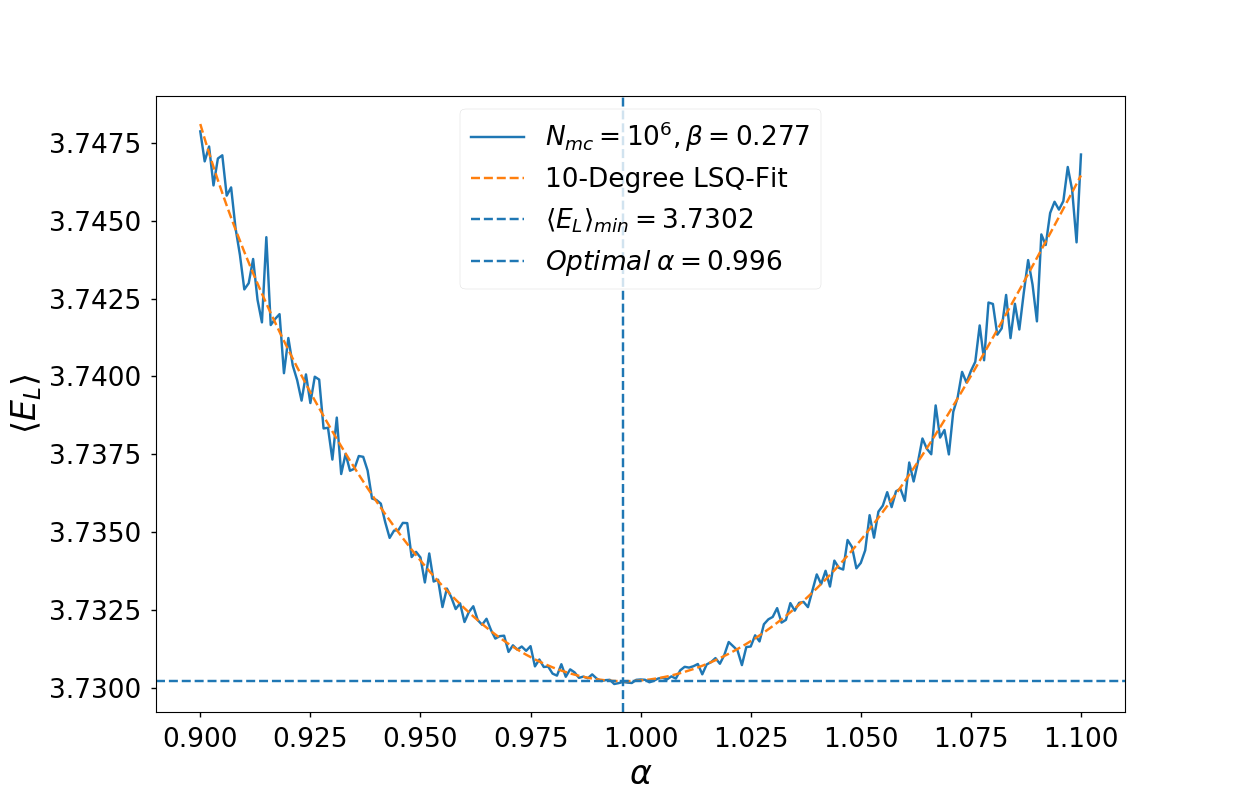
\includegraphics[scale=0.30]{figsPartII/run6.png}
\caption{Caption.}
\label{IIfig3}
\end{figure}

where the optimal variational parameters for $\Psi_{T2P}$ are $\beta = 0.277$ and $\alpha = 0.996$.\par
Now repeating the computation of the mean distance $r_{12}$ for the optimal variational parameters.

\begin{table}[H]
\center
\caption{Mean distances $r_{12}$ for perturbed Hamiltonians for $\Psi_{T2}$ under varying frequencies $\omega$.}
\begin{tabular}{| p{2cm} | p{2cm} |}
\hline
$\omega$ & $r_{12}$\\
\hline
$0.001$ & $17.65$ \\
\hline
$0.5$   & $\phantom{1}2.60$ \\
\hline
$1.0$   & $\phantom{1}1.81$ \\
\hline
\end{tabular}
\label{TablePII}
\end{table}

\subsection{Part III: }
The ratios (ratio) is computed in the frequency range $\omega \in \{0.01, 1.0\}$ with a step size $h_\omega=0.05$, starting from and including $0.05$. Thus keeping the result for $\omega=0.01$.

\begin{figure}[H]
\center
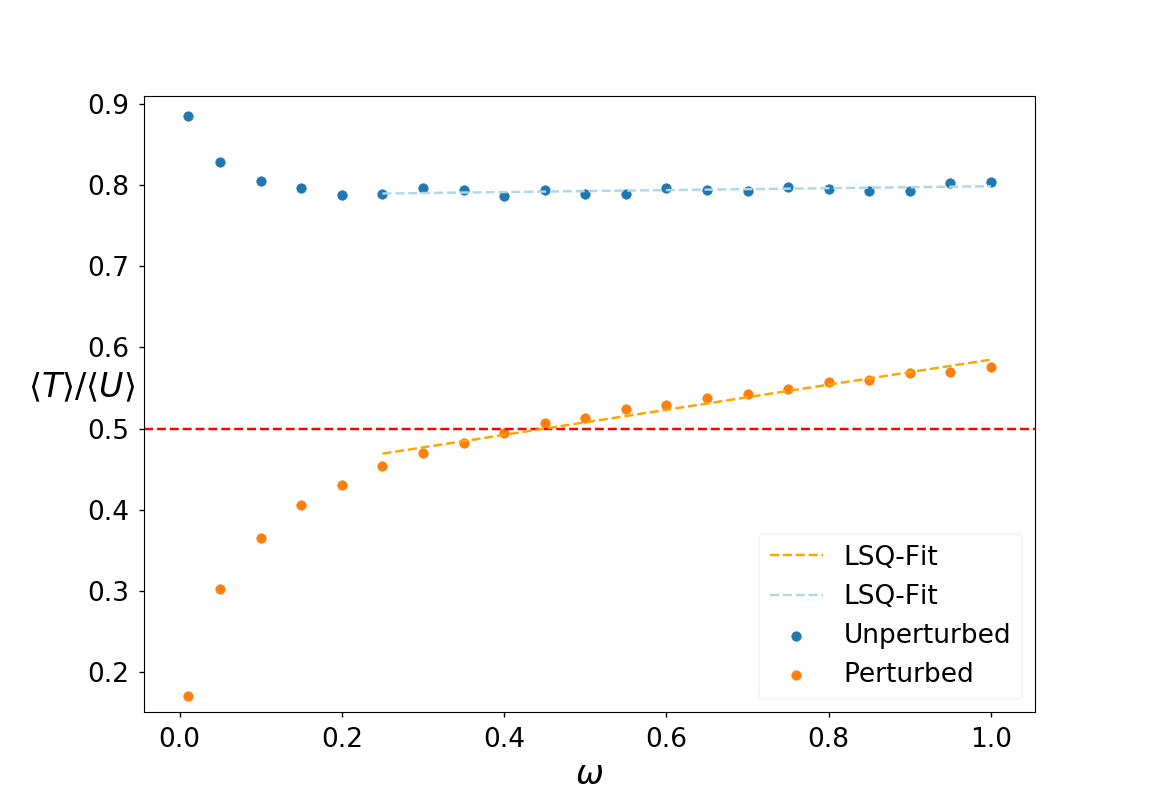
\includegraphics[scale=0.32]{figsPartIII/ratios.png}
\caption{Caption.}
\label{IIIfig1}
\end{figure}

with a least squares fitting in appropriate interval of frequencies. Adding a plot with the associated distances

\begin{figure}[H]l
\center
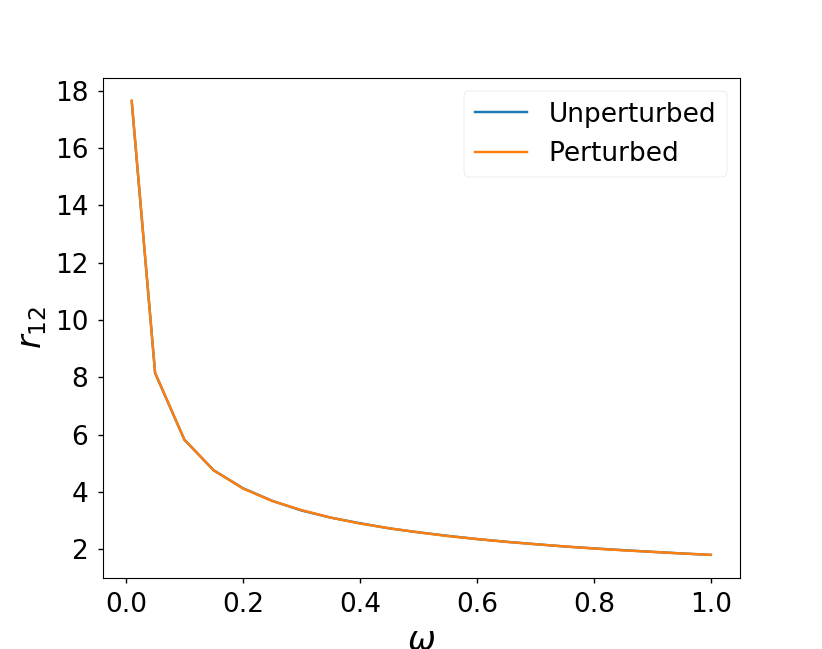
\includegraphics[scale=0.4]{figsPartIII/distances.png}
\caption{Caption.}
\label{IIIfig2}
\end{figure}


\section{Discussion}

\subsection{Part I:}
The VMC computations start becoming stable after about $10^4$ Monte Carlo cycles, which is seen in plot (\ref{Ifig1}), which is due to the curves having a well defined minima at this cycle number. The same, however, cannot be argued for the variance following in plot (\ref{Ifig2}). The smoothness of the variance is thus a better measure for the stability. Which is seen as to begin to happen at cycle numbers greater than $10^4$.\par
Further increases in cycle number $10^{i>4}$, $i=5,6,7$, as shown in (\ref{Ifig3}) tend the local energy and variance curves to be increasingly smooth. Thus choosing the cycle number $10^6$ seems like a satisfying choice when it comes to both numerical stability and computational efficiency.\par
Since the exact solution for the unperturbed ground state energy of trial function $\Psi_{T1}$ is $\mathcal{E}=3.0$, it is shown from table (\ref{resItable1}) that the minima of the local energy, which is the approximated ground state energy is equal to $3.0000\pm 10^{-4}$ for cycle numbers $10^{i>4}$. Comparing this to the eigenvalue computations made in the author's report \cite[pg.6]{Project2} uncaptioned table just above table IV. The ground state energy of a buckling beam system, was computed to be $\lambda_0 = 1.499$ for a number of computed eigenvalues $N=110$. This is analogous to referring to high accuracy with high cycle number in this report. This constitutes a solution to the relative coordinate eigenvalue problem in this report, thus the center of mass energy must also be added. Which is equal to $1.5 a.u$, thus giving a difference between the results of $10^{-3}$ which is a relatively good agreement. When it comes to the result yielded by the VMC method, it gives the exact result for the unperturbed Hamiltonian, stable at $10^{i\geq 5}$ cycles.\par
Furthermore, for the perturbed Hamiltonian, again referring to the results of $\omega=1.0$ from earlier project 2 \cite[pg.6]{Project2} table V. The eigenvalue for the relative coordinate is computed to be $4.1$, which with added center of mass energy yields $5.5$. There is cause for concern regarding this result, however, due to the fact that the process of extending the jacobi eigenvalue solver was not very rigourus. Not for testing nor with sufficient trials of various tolerances with the J-eigen-solver. Comparing both of these values to the exact analytical value of $3.588$ means the result of the VMC computation for $\Psi_{T1}$ is the most accurate at $3.773\pm 10^{-3}$. \par
The differences in the mean distances for the perturbed/unperturbed Hamiltonian shows a global, for the computed frequency interval, increase in $r_{12}$ for the unperturbed case. For larger frequencies, however, the mean distances seem to converge. This seems to imply that for weaker harmonic oscillator strengths, the more significant is the electron-electron repulsion.

\subsection{Part II:}
Initially, the first variational run (\ref{IIfig1}), for $\Psi_{T2}$ under fixed $\alpha=0.9$ yields an improved result over $\Psi_{T1}$, as quantified

\begin{equation}
\frac{3.773-3.74036}{E_{gs}=3.558}\approx 1\%
\end{equation}

The further alternating optimization process of the variational parameters $\alpha$ and $\beta$ leads eventually to the final result of the VMC $E_{gs} \approx \langle E_L\rangle_{min}=3.7302$, which in turn further increases the improved result by an additional $\approx 0.2\%$. This seems to imply that the significance of accounting for the cusp condition by applying the Jastrow factor is quantified, can be quantified by the $1.2\%$ improvement.	\par

Comparing table (\ref{TablePII}) with (\ref{TablePartI}) it is clear that the second trial function $\Psi_{T2}$ results in an even larger relative distance between the electrons for the ground state. From an electromagnetic point of view, this can be interpreted as the first trial function not taking into account the significance of the Coulomb interaction between the electrons. 	Taking the ratios of the mean distances in table (\ref{TablePII}) with the perturbed values in table (\ref{TablePartI}), referred to as the new ratio; and comparing that to the ratios of the perturbed and unperturbed values in the latter table. These ratios seem to partly support the notation discussed in part I that there is a higher significance to the e-e repulsion with weaker field strengths. The ratios for $\omega = 1.0$ are approximately unchanged, while the new ratio is lower for the weaker field $\omega = 0.01$ than for $\omega =0.5$. This seems to modify the implication of part I to, yes, the mean distances seem to converge for larger frequencies $\omega=1.0$, but the significance of the e-e repulsion for the trial function 2 is higher at around $\omega=0.5$.

\subsection{Part III: }
The specialized Virial theorems listed in (\ref{sec:TheoryVirial }) are for system where the total potential energy reflects a force between the particles which scale proportionally with the distance to the power of some degree.\par
Firstly the first trial function held up quite well to the virial theorem under the unperturbed case

\begin{table}[H]
\center
\caption{Expectation values of kinetic and potential energies of $\Psi_{T1}$ under perturbed and unperturbed conditions. Data found in \textit{SavedResults/Bulk2/} files \textit{datOmegasT1P and datOmegasT1U}, fourth and fifth columns. Counting from 1.}
\begin{tabular}{| p{2cm} | p{1.5cm} | p{1.5cm} | p{1.5cm} |}
\hline
 & $\langle T \rangle$ & $\langle U \rangle$ & $\omega$ \\
 \hline
Unperturbed & $0.015$ & $0.014$ & $0.01$ \\
\hline
	& $0.749$ & $0.750$ & $0.5$\\
\hline
 & $1.495$ & $1.504$ & $1.0$\\
 \hline
Perturbed & $0.013$ & $0.092$ & $0.01$ \\
\hline
	& $0.673$ & $1.370$ & $0.5$\\
\hline
 & $1.495$ & $2.416$ & $1.0$\\
 \hline 
\end{tabular}
\end{table}

while as seen, the perturbed case didn't hold up. \par 
This seems to be somewhat of a similar for the trial function $\Psi_{T2}$, shown in plot (\ref{IIIfig1}). The unperturbed case seems keeps an approximately constant ratio of about for the frequency interval $\omega \in \{0.25,1.0\}$. According to the LSQ-fitting, however, the ratio increases with a slope of $\sim 0.01$. The perturbed case shows a logarithmic behaviour; or, if restraining to the same frequency interval, an approximately linear increase with a slope of $0.15$. The plot shows, for the unperturbed case, that at the frequency $\omega\approx 0.42$ the ratio of kinetic and potential energy is $0.5$, meaning it is approximately behaving like a system only affected by e-e repulsion. Meaning that it is the dominating force. If the trend of liear increase is assumed to hold and perhaps stabilize at the ratio of $1.0$, then the dominating force will be the harmonic oscillator potential. Another way of seeing this is to also bring the mean distances into the interpretation. Plot (\ref{IIIfig2}) shows the mean distance going as $1/r$ as a function of frequencies. Meaning that the stronger the harmonic oscillator potential strength is, the smaller distance between the electrons. This supports the notion of the system behaving more and more like a pure harmonic oscillator for increased field strengths.


\section{Concluding Remarks}
The VMC-computational results are summarized for the parts of this report.\par
It was discovered in part I that a general threshold for thermalization was for cycle numbers greater than or equal to $10^4$, however in pursuit of a balance between higher precision and computational efficiency, the main results were computed with a cycle number of $10^6$. Furthermore it was found that the first trial function without accounting for the cusp-condition gave an approximation to the unperturbed ground state energy, which agreed with the exact ground state energy of $3.0$ to a $100\%$ degree of accuracy. The perturbed ground state energy, was found to deviate from the exact ground state energy of $3.588$ with about $5.7\%$.\par
In part II it was found, by the second trial wavefunction and a interchanging variational proceedure of two variational parameters, that the deviation of the approximated ground state energy could be reduced to $4.62\%$, which yields the significance of the Jastrow factor to be about $1.1\%$ degree of accuracy.\par
The main findings of part III were that for, and close to, the frequency $\omega=0.42$, the dominating force is the e-e repulsion, while for larger $\omega>1.0$ the system tends to be more and more approximated by a pure harmonic oscillator.

\section{Author's Remarks}


\section{Github-Repository}
\url{https://github.com/nhofield/fys3150Projects.git}
The programs for this report are found in the folder named, Prosjekt 4.

\begin{thebibliography}{9}

\bibitem{McMillanPaper}
  William L. McMillan,
  \emph{\LaTeX: Ground State of Liquid $He^4$}.
  \url{https://journals.aps.org/pr/abstract/10.1103/PhysRev.138.A442}
\bibitem{VirialTheoremProof}
	P. Gutierrez,
	\emph{\LaTeX: University of Oklahoma, Lecture Notes in Classical Mechanics, Lecture 14}
	\url{http://www.nhn.ou.edu/~gut/notes/cm/lect_14.pdf}

\bibitem{Project2}
	Noah D. Oldfield,
	\emph{\LaTeX: Writing an Eigenvalue Solver which can be applied to Scaled Differential
Equations}
	\url{https://devilry.ifi.uio.no/devilry_group/student/535982/feedbackfeed/}

\bibitem{Project4}
	Noah D. Oldfield,
	\emph{\LaTeX: Simulating the Ising Model by the Applied Metropolis-Algorithm}
	\url{https://devilry.ifi.uio.no/devilry_group/student/550709/feedbackfeed/}

\bibitem{Griffiths}
	David J. Griffiths,
	\emph{\LaTeX: Introduction To Quantum Mechanics, Second Edition}

\bibitem{Zettili}
	Nouredine Zettili,
	\emph{\LaTeX: Quantum Mechanics, Concepts and Applications}

\bibitem{LectureNotes}
	Morten H. Jensen,
	\emph{\LaTeX: Computational Physics FYS3150, lecture notes 2015}
	\url{https://github.com/CompPhysics/ComputationalPhysics/blob/master/doc/Lectures/lectures2015.pdf}

\end{thebibliography}
	
\end{document}
%
% ****** End of file aipsamp.tex ******